\documentclass{VUMIFPSbakalaurinis}
\usepackage[table]{xcolor}
\usepackage{algorithmicx}
\usepackage{algorithm}
\usepackage{algpseudocode}
\usepackage{amsfonts}
\usepackage{amsmath}
\usepackage{bm}
\usepackage{caption}
\usepackage{color}
\usepackage{float}
\usepackage{graphicx}
\usepackage{listings}
\usepackage{subfig}
\usepackage{wrapfig}
\usepackage{tikz}

\usepackage{enumitem}
\setitemize{noitemsep,topsep=0pt,parsep=0pt,partopsep=0pt}
\setenumerate{noitemsep,topsep=0pt,parsep=0pt,partopsep=0pt}

% Ignore all trivial warnings
\hbadness=5000
% Titulinio aprašas
\university{Vilniaus universitetas}
\faculty{Informatikos institutas}
\department{Programų sistemų katedra}
\papertype{Bakalauro baigiamasis darbas }
\title{Rodiklių duomenų apdorojimo sistemų generavimas iš duomenų modelių}
\titleineng{Generation of Indicator Data Processing Systems\\from Data Models}
\author{Vytautas Žilinas}
\supervisor{lekt. Andrius Adamonis}
\reviewer{assoc. prof., dr. Karolis Petrauskas}
\date{Vilnius – \the\year}

% Nustatymai
% \setmainfont{Palemonas}   % Pakeisti teksto šriftą į Palemonas (turi būti įdiegtas sistemoje)
\bibliography{bibliografija}

\begin{document} 
\maketitle

\cleardoublepage\pagenumbering{arabic}
\setcounter{page}{2}

\sectionnonumnocontent{Santrauka}
Šį darbą sudaro teorinė ir eksperimentinė dalys. Teorinėje dalyje apibrėžiamas rodiklis, jo struktūra ir struktūros pokyčiai. Apibrėžiami kokie yra įmanomi pokyčiai ir kaip eksperimentinėje dalyje kuriamas sprendimas prie pokyčių prisitaikys. Specifikuojama duomenų struktūra ir duomenų struktūrų apjungimo ir skirtumo operacijas. Apibrėžiamas srautinis apdorojimas ir pasirenkama sistema, kuri bus naudojama eksperimentinėje dalyje. Remiantis gautais rezultatais
nustatoma, kad šiam uždaviniui spręsti pasirenkama "Heron" srautinio apdorojimo sistema. Remiantis pasirinkta srautinio apdorojimo sistema ir apibrėžta rodiklių duomenų struktūra, eksperimentui nusprendžiama generuoti srautinio apdorojimo modulius parašytus "Python" programavimo kalba. Eksperimentinėje dalyje remiantis pasiūlyta architektūra realizuojama bandomoji sistemos versija. Atliekant skirtingų kiekių rodiklių duomenų ir rodiklių duomenų pokyčių simuliaciją stebėjimais analizuojamas šios sistemos tinkamumas apibrėžtam uždaviniui spręsti. Gauti tyrimų rezultatai lyginami, pateikiamos išvados. Taip įrodoma, kad toks sprendimas gali būti įgyvendinamas ir kad kodo generavimas ir srautinio apdorojimo sistema "Heron" yra tinkamas sprendimas kintančių rodiklių uždaviniui spręsti.
\raktiniaizodziai{srautinis apdorojimas, kodo generavimas, rodiklis, rodiklio duomens pokyčiai}   

\sectionnonumnocontent{Summary}
This work consists of a theoretical and an experimental part. Theoretical part defines the indicator, its structure and changes in indicator structure. It define what changes are possible and how the developed solution in the experimental part will adapt to the changes, specifies the data structure and data structure merging and difference operations, defines stream processing and selects the system to be used in the experimental part. Based on the results it is determined that "Heron" stream processing system is chosen to solve this task. Based on the selected stream processing system and the defined data structure of indicator, it is decided to generate streaming modules written in "Python" programing language. In the experimental part, a pilot version of the system is implemented based on the proposed architecture. By doing the simulation using varying amounts of indicators and indicator changed, the suitability of this system for a defined task is tested. The results of this research are compared and conclusions are given. This demonstrates that such a solution can be implemented and that the code generation and streaming system "Heron" is the right solution to deal with the challenge of changing indicators.
\keywords{stream processing, code generation, indicator, indactor structure change}

\tableofcontents

\sectionnonum{Įvadas}
 
Šiame darbe yra nagrinėjamas rodiklių duomenų apdorojimas ir kuriamas koncepcinis sprendimas galintis prisitaikyti, kai keičiama rodiklių duomenų struktūrą. Rodiklių duomenimis vadinkime pasikartojančių įvykių parametrus aprašančius duomenis. Pavyzdžiui, įvairių matuoklių – temperatūros, resursų suvartojimo – fiksuojamus rodmenis, kasmėnesinius veiklos indikatorius, tokius kaip veiklos finansines ataskaitas ar veiklos procesų indikatorius. Taip pat rodiklių struktūra gali keistis laikui bėgant: objektų atributų taksonomija (pvz. mirties priežasčių sąrašas, finansinių sąskaitų sąrašas) arba įrašo atributų sąrašai. Surenkamu rodiklių duomenų kiekis visada didėja, taip pat ir duomenų kiekis, kuriuos reikia apdoroti pagal rodiklius auga, todėl standartiniai sprendimai, pavyzdžiui, reliacinės duomenų bazės netinka dėl ilgos apdorojimo trukmės. Rodiklių duomenų bazės pasižymi tuo, kad duomenys į jas patenka iš daug skirtingų tiekėjų ir patekimo laikas tarp tiekėjų nėra sinchronizuojamas, o suagreguotą informaciją vartotojai gali užklausti bet kurio metu. Todėl šiame darbe bus nagrinėjamas srautinis duomenų apdorojimas, kuris patenkančius duomenis apdoros realiu laiku, ir saugos jau apdorotus. \par
Realaus laiko duomenų apdorojimas (angl. Real-time data processing) yra jau senai nagrinėjamas, kaip vienas iš būdų apdoroti didelių kiekių duomenis (angl. Big data). Vienas iš realaus laiko apdorojimo sprendimų yra srautinis duomenų apdorojimas. Srautinis duomenų apdorojimas (angl. stream processing) – lygiagrečių programų kūrimo modelis, pasireiškiantis sintaksiškai sujungiant nuoseklius skaičiavimo komponentus srautais, kad kiekvienas komponentas galėtų skaičiuoti savarankiškai \cite{shortstreamproc}. Darbe yra analizuojamos jau egzistuojančias srautinio apdorojimo sistemų programas pagal srautinio apdorojimo programų savybes aprašytas Michael Stonebraker, pasirenkama vieną srautinio apdorojimo programa ir pagal ją sukuriamas koncepcinis sprendimas. 
\par
Kadangi rodikliai laikui bėgant gali būti keičiami reikia, kad sprendimas, galėtų prisitaikyti prie pokyčių. Yra keli būdai kaip tai tokie sprendimai gali būti kuriami:
\begin{itemize}
    \item Rankinio atnaujinimo sprendimas. Sukuriamas sprendimas pagal esamus reikalavimus, o atsiradus naujiems reikalavimams būtų kuriamos naujos arba keičiamos esamas apdorojimo sistemos. 
    \item Universalus sprendimas. Sukuriamas universalus parametrizuojamas sprendimas ir pritaikomas užduotims nustatant parametrus.
    \item Kodo generavimo sprendimas. Sukuriamas sprendimas, kuris generuoja srautinio duomenų apdorojimo sistemas pagal iš anksto aprašytą struktūrą.  
\end{itemize}   
Tinkamas sprendimas turi būti išrinktas pagal sprendžiamą problemą. Jei nėra numatomas kitimas, pagal ką turi būti apdorojami duomenys, tai galima pasirinkti ir rankinio apdorojimo sprendimą, kadangi nėra didelės tikimybės, kad teks keisti sprendimą. Toks sprendimas tiktų apdorojant išmaniųjų skaitiklių duomenis \cite{skaitikliai}. Universalus sprendimas taip pat gali būti tinkamas jei pirminiai rodiklių duomenis yra specifiški ir yra poreikis juos visus apdoroti. Toks sprendimas gali būti aktualus apdorojant duomenis iš sensorių, kurie matuoja namų būsena (temperatūra, drėgmę ir t.t.) ir bet koks naujas sensorius taip pat turi būti prijungtas ir apdorotas \cite{yang2017iot}. Šiame darbe buvo norima nagrinėti kodo generavimo sprendimo tinkamumą užduotims. \par
Pagal Jack Herrington 2003 metų knygą "Code Generation in Action" kodo generavimas - tai rašymas programinės įrangos, kuri rašys reikiamą programinę įrangą problemai spręsti. Tai daroma tokiais atvejais, kai sprendžiama problema reikalauja daug rankinio darbo, kurį įmanoma automatizuoti. Kuo didesnio sprendimo reikalauja uždavinys tuo patraukliau tampa naudoti kodo generavimą sprendimo kūrimui. Kodo generavimas suteikia tokius privalumus: 
\begin{itemize}
    \item Architektūrinį nuoseklumą: 
    \begin{itemize}
        \item Verčia programuotojus labiau mąstyti apie architektūrą.
        \item Jei sunku "priversti" generatorių generuoti reikiamą kodą, problema gali būti architektūroje.
        \item Geros dokumentacijos buvimas sumažina problemą, kai nariai palieką projektą.
    \end{itemize}
    \item Abstrakciją:
    \begin{itemize}
        \item Programuotojai galės kurti naujus šablonus, kurie leis esamą funkcionalumą pritaikyti kitomis kalbomis, sprendimais daug paprasčiau negu rankomis parašytą kodą.
        \item Verslo analitikai gali apžvelgti ir patvirtinti sprendimo abstrakciją.
        \item Abstrakcija padės paprasčiau paruošti dokumentacija, testavimo atvejus, produkto palaikymo medžiagą ir t.t.  
    \end{itemize}
    \item Aukštą komandos moralę - rašomas kodas bus nuoseklus ir kokybiškas todėl kels komandos pasitikėjimą.
    \item Tinkamas sprendimas Judriajam programavimui, kadangi kodo generavimo kuriami sprendimai yra lankstesni, tai leidžia ateityje juos lengviau keisti ir atnaujinti.   
\end{itemize} 
Kodo generavimas tampa tikrai naudingas tada, kai jis naudojamas didelių kiekių rankiniam kodavimui pakeisti \cite{herrington2003code}. \par
Darbe nagrinėjamas architektūra ir koncepcinis sprendimas generuojantis srautinio apdorojimo sistemas pagal rodiklių duomenų modelius. Rodiklių duomenis apdorojantis koncepcinis sprendimas turi pasižymėti tokiomis savybėmis: 
\begin{itemize}
    \item Srautinių apdorojimo sistemų generavimas pagal deklaratyvų aprašymą.
    \item Galimybė keisti esamas apdorojimo sistemas, kai pakeičiamas rodiklių duomenų modelis.
    \item Išvestinių rodiklių gavimas iš daugiau nei vieno rodiklio transformacijos.
    \item Išvestinių rodiklių apdorojimas pagal iš anksto apibrėžtas funkcijas.
\end{itemize}  

Tikslas: Sukurti rodiklių duomenų srautinio apdorojimo sistemos, pritaikomos prie duomenų struktūrų naudojant kodo generavimą, architektūrą.

Uždaviniai:
\begin{enumerate}
    \item Apibrėžti rodiklių duomenų modelį ir galimus rodiklių duomenų struktūros pokyčius.
    \item Atlikus šaltinių analizę pasirinkti srautinio duomenų apdorojimo sprendimą.
    \item Sudaryti srautinio apdorojimo sistemos architektūrą, pagal ją sukurti koncepcinį sprendimą. 
    \item Nustatyti sukurto koncepcinio sprendimo ir architektūros savybes atliekant bandymus su rodiklių duomenimis.
\end{enumerate}

\section{Rodiklių duomenys}

Rodiklių duomenys - pasikartojančių įvykių parametrus aprašančius duomenys. Rodiklių duomenys pasižymi tuo, jog tik surinkti ir apdoroti tampa aktualus. Taip pat rodikliai yra nepastovūs, jų struktūra gali būti keičiama - atsirasti naujų savybių, kurias reikia surinkti arba yra pašalinamos jau esamos savybės. Rodiklių duomenys yra renkami ir analizuojami labai skirtingiems poreikiams - visur kur reikalinga statistika ir apdorojami didelį kiekiai duomenų yra naudojami rodikliai: tai gali būti įmonės vedamą "Microsoft Excel" skaičiuoklė, kurioje užrašyta kiek buvo mokėta už elektrą kiekvienais metais per paskutinius 10 metų arba juodosios skylės nuotrauka padaryta koreliuojant didelio duomenų kiekį iš 8 skirtingų teleskopu ir gauti rodikliai rodo taškus ant paveikslėlio, kurio dydis yra \(10^{12}\) kartų mažesnis nei pradiniai duomenys \cite{akiyama2019first}.

\subsection{Pirminiai rodiklių duomenys}

Rodiklių duomenys yra gaunami apdorojus pirminius rodiklių duomenis, kurie susidaro iš raktų ir reikšmių žodyno (\ref{img:duomenys} pav.), kur raktas gali būti tik tekstinio tipo, o reikšmė - tekstas arba skaičius. Pirminių rodiklių duomenų raktai ir raktų kiekis gali nesutapti - žodynai gali turėti daugiau raktų arba žodyno reikšmės gali būti nereikalingos einamojo rodiklio išskaičiavimui. \par 
Kadangi pirminiai rodiklių duomenys gali būti gaunami iš skirtingų šaltinių, skirtingais laikais, todėl kuriamas sprendimas turi galėti priimti duomenis asinchroniškai ir iš skirtingų šaltinių, o sprendimas realiu laiku turi sugebėti apdoroti reikiamus duomenis, o nereikalingus atmesti. 

\begin{figure}[H]
    \centering
    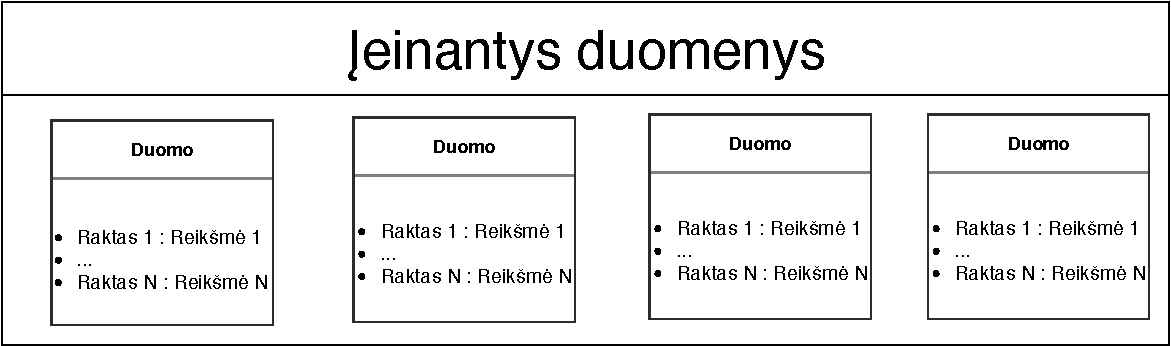
\includegraphics[width=1\textwidth]{img/duomenys.pdf}
    \caption{Pirminiai rodiklių duomenys}
    \label{img:duomenys}
\end{figure}

\subsection{Rodiklių duomenų modelis}

Norint apdoroti daug skirtingų rodiklių apsibrėžiamas bendrą rodiklių duomenų modelį (\ref{img:rodiklio_apibrezimas} pav.), pagal kurį bus generuojamos srautinio duomenų apdorojimo sistemos. Siūlomas apibrėžimas susidaro iš trijų dalių: 
\begin{itemize}
    \item Rodiklių duomenų pirminis raktas sudarytas iš pirminių rodiklių duomenų raktų rinkinio.
    \item Pirminių rodiklių duomenų reikšmių srities apribojimai.
    \item Rodiklių. 
\end{itemize}

\begin{figure}[H]
    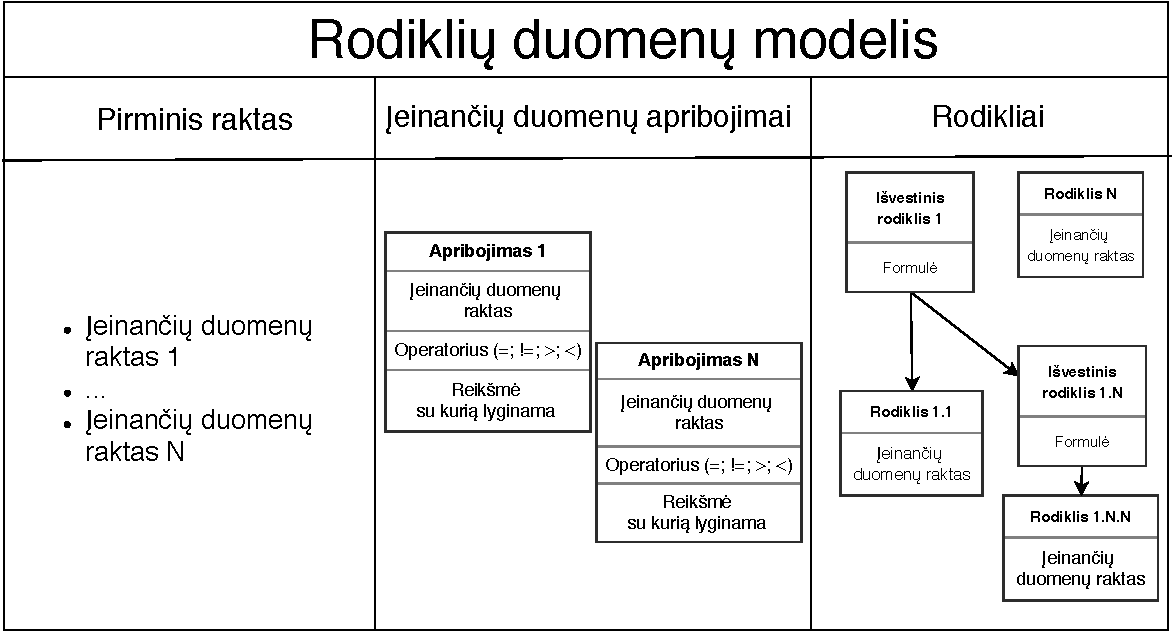
\includegraphics[width=1\textwidth]{img/rodiklio_modelis.pdf}
    \caption{Rodiklių duomenų modelis}
    \label{img:rodiklio_apibrezimas}
\end{figure}

\subsubsection{Pirminis raktas}

Pirma rodiklio apdorojimo apibrėžimo dalis nusako raktų rinkinį reikšmių pagal kurias grupuojami apdoroti duomenis. Pavyzdžiui:
\begin{itemize}
    \item Statistikos srityje: norint surinkti duomenis aprašančius \textbf{skirtingų savivaldybių} nekilnojamo turto kainas pagal \textbf{metus}, raktų rinkinys atrodys taip: \[\{\textit{"Savivaldybė", "Metai"}\}\]
    \item Sensoriniai rodikliai: norint surinkti vienos dienos duomenis aprašančius \textbf{skirtingų sensorių} parodymus \textbf{kiekvieną valandą}, \textbf{kiekvienam ofiso kabinetui}, raktu rinkinys atrodys taip: \[\{\textit{"Sensoriaus tipas", "Valanda", Kabineto Numeris}\}\] 
    \item Buhalterijoje: norint surinkti duomenis parodančių kiek ir \textbf{kokie skyriai} patyrė išlaidų kiekvieną šių \textbf{metų mėnesį}, raktų rinkinys atrodys taip: \[\{\textit{"Skyriaus pavadinimas", "Mėnesis"}\}\] 
\end{itemize}  \par
Raktų kiekis neturi būti ribojamas, kadangi realiame pasaulyje yra neribotas kiekis duomenų pagal kuriuos galima grupuoti. Visų raktų reikšmių kiekių sandauga - apdorotų rodiklių duomenų pirminių raktų aibė. 

\subsubsection{Pirminių rodiklių duomenų apribojimai}

Antra rodiklio duomenų modelio dalis susidaro iš rinkinio apribojimų, kurie aprašo kokie duomenys turi būti apdorojami. Apribojimai yra aprašomi predikatais.
Pavyzdžiui:
\begin{itemize}
    \item Statistikos srityje: norint surinkti žmonių, \textbf{vyresnių nei 60 metų} atlyginimus pagal kalendorinius metus, apribojimų sąrašas atrodys taip: \[\textit{"Amžius" > 59}\]
    \item Sensoriniai rodikliai: norint surinkti \textbf{tik savaitgalio} sensorių rodiklius, apribojimų sąrašas atrodys taip: \[\textit{"Savaitės Diena" > 5}, \textit{"Savaitės Diena" < 8}\]
    \item Buhalterijoje: norint apdoroti tam tikrus duomenis \textbf{tik "Marketingas" skyriaus} apribojimų sąrašas atrodys taip: \[\textit{"Skyriaus pavadinimas" == "Marketingas"}\] 
\end{itemize}  
Apribojimų kiekis yra neribojamas. Šie apribojimai turi leisti naudoti tuos pačius duomenis skirtingiems rodikliams ir rodiklių rinkiniams apdoroti. Pirminiai rodiklių duomenys turi būti ribojami pagal reikšmes, kurios turi priklausyti apribojimų aibių sankirtai. Jei yra pateikti du apribojimus, tai pirminio rodiklio duomens ribojamos reikšmės turi patekti į abiejų apribojimų aibes. 
\par

\subsubsection{Rodikliai}

Ši rodiklių duomenų modelio dalis sudaryta iš dviejų skirtinų tipų komponentų:
\begin{itemize}
    \item Rodiklis - iš pirminių rodiklių duomenų gaunami parametrai. Rodiklių duomenų modelyje rodiklis yra sudarytas iš pavadinimo ir pirminių rodiklių duomenų rakto.
    \item Išvestinis rodiklis - iš vieno ar daugiau rodiklių išskaičiuojami parametrai. Rodiklių duomenų modelyje išvestinis rodiklis yra sudarytas iš pavadinimo ir rodiklių, nuo kuriu priklauso išvestinis rodiklis, transformacijos aprašo - formulės. 
\end{itemize}
Rodiklių duomenų modelyje komponentų priklausomybės sudaro priklausomybių medį, kurio viršūnės - rodikliai, o keliai - priklausomybės tarp rodiklių. Priklausomybių medyje kabančios (galinės) viršūnės visada bus rodiklio tipo, o visos kitos išvestinių rodiklių tipo.
Pavyzdžiui:
\begin{itemize}
    \item Statistikos srityje: norint surinkti rodiklių duomenis nekilnojamo turto kainų ir žmonių kaitos šalyje (\(\textit{Žmonių kaita} = (\textit{Gimstamumas - Mirtingumas}) + (\textit{Migracija} * \textit{Gyventojų kiekis}\)), renkamų rodiklių medžiai apsirašytų taip: 
    \[	
        
\begin{tikzpicture}[sibling distance=7em, every node/.style = {shape=rectangle, rounded                                corners, draw, align=center,	
            top color=white, bottom color=white}]	
            \node{Nekilnojamo turto kaina};
        \end{tikzpicture} 
    \]
    \[
        \begin{tikzpicture}[sibling distance=10em,
            level distance=2cm,
            every node/.style = {shape=rectangle, rounded corners,	
                                 draw, align=center,	
                                 top color=white, bottom color=white}]	
            \node{Žmonių kaita\\Nuolatinė kaita + (Migracija * Gyventojų kiekis)}
                    child { node {Nuolatinė kaita\\Gimstamumas - Mirtingumas} 
                            child {node {Mirtingumas}}
                            child {node {Gimstamumas}} }	
                    child { node {Migracija} } 	
                    child { node {Gyventojų kiekis} }; 	
        \end{tikzpicture} 	
    \]
    \item Sensoriniai rodikliai: norint surinkti drėgmės, temperatūros ir šviesos sensorių rodiklius, rodiklių medžiai atrodys taip:
    \[	
        
\begin{tikzpicture}[sibling distance=7em,  every node/.style = {shape=rectangle,  
                                rounded corners, draw, align=center,	
                                top color=white, bottom color=white}]	
            \node{Drėgmė};
        \end{tikzpicture}\>\>\>\>
        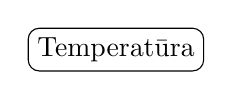
\begin{tikzpicture}[sibling distance=7em, every node/.style = {shape=rectangle, 
                                rounded corners, draw, align=center,	
                                top color=white, bottom color=white}]	
            \node{Temperatūra};
        \end{tikzpicture}\>\>\>\>
        
\begin{tikzpicture}[sibling distance=7em, every node/.style = {shape=rectangle, rounded                                corners, draw, align=center,	
                                top color=white, bottom color=white}]	
            \node{Šviesa};
        \end{tikzpicture} 	
    \]
    \item Buhalterijoje: norint suskaičiuoti kiek įmonės darbuotojai gauna pajamų (\(\textit{Pajamos} = (\textit{Atlyginimas}/1.7) + \textit{Premijos}\)) rodiklių medis bus toks: 
    \[	
        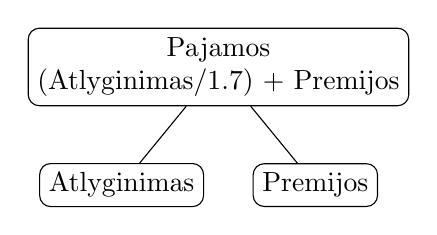
\begin{tikzpicture}[sibling distance=7em,	
            every node/.style = {shape=rectangle, rounded corners,	
                                 draw, align=center,	
                                 top color=white, bottom color=white}]	
            \node {Pajamos\\(Atlyginimas/1.7) + Premijos}	
                    child { node {Atlyginimas} }	
                    child { node {Premijos} } ;	
        \end{tikzpicture} 	
    \]
\end{itemize}  


\subsection{Rezultatų struktūra}

Apdorotų rodiklių rezultatai gauti iš pirminių rodiklių duomenų gali būti užrašyti lentelę. Lentelės duomenų pirminis raktas yra sudarytas iš pirminių rodiklių duomenų reikšmių kombinacijos gautos pagal rodiklio modelio pirminį raktą. Rezultatų lentelės stulpeliuose aprašytas pirminis raktas ir išvestiniai rodikliai. Rezultatų lentelės išvestinių rodiklių kolonėlės susidaro iš apdorotų rodiklių duomenų.

\begin{figure}[H]
    \centering
    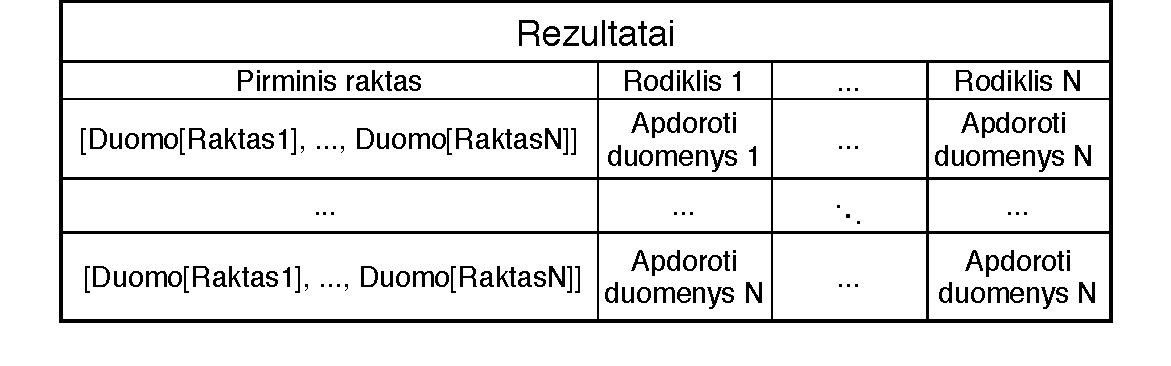
\includegraphics[width=1\textwidth]{img/rezultatai.pdf}
    \caption{Rezultatų struktūra}
    \label{img:rezultatai}
\end{figure}

\subsection{Rodiklių duomenų struktūros kitimas}

Rodiklių duomenų struktūra gali būti keičiama laikui bėgant. Buhalterijos srityje tai gali įvykti dėl naujo įstatymo, kuris pakeičia tam tikrų rodiklių išskaičiavimą. Išmaniuosiuose namuose tai gali būti naujas išmaniųjų namų sensorius. Statistikos srityje tai gali būti poreikis išskaidyti tam tikrus rodiklius į mažesnius rodiklius -  rinkti ne migracijos rodiklį kaip vieną, o atskirai emigraciją ir imigraciją. \par
Šiame darbe rodiklių duomenų struktūrų pokyčiai apribojami taip:
\begin{itemize}
    \item Pirminis raktas negali keistis, nes naujos reikšmės tampa nepalyginamos su anksčiau surinktomis. Tarkim buvo renkami rodikliai metinių duomenų, o pagal poreikius reikia rinkti mėnesinius duomenis, ir lyginimas su anksčiau surinktais tampa neįmanomas. Todėl bet kokius pirminio raktus pokyčius turi būti laikomi nauju rodikliu. 
    \item Apribojimai gali keistis, tačiau šie pokyčiai turi būti naudojami tik tam, kad būtų išlaikytos pradinės apdorojamų pirminių rodiklių duomenų aibės. Tarkime yra poreikis apdoroti duomenis iš visų skyrių išskyrus administraciją ir tokiam uždaviniui buvo sukurtas apribojimas - \(\textit{"Skyriaus pavadinimas" != "Administracija"}\). Tačiau po laiko dalis administracijos skyriaus atsiskyrė ir susikūrė naujas HR skyrius. Siekiant, kad būtų išlaikyta apdorotų rodiklių lyginimo prasmė, nauji apribojimai atrodys taip: \(\textit{"Skyriaus pavadinimas"!="Administracija"}, \textit{"Skyriaus pavadinimas"!="HR"}\)
    \item Rodikliai ir išvestiniai rodikliai gali būti keičiami - nauji rodikliai pridedami, o seni pašalinami. Šie pokyčiai gali būti daromi bet kurioje rodiklių tarpusavio priklausomybės medžio vietoje. Rodiklių pokyčiai neturi daryti įtaką kitų rodiklių skaičiavimams. Tarkime, jog  pajamas skaičiuojamos naudojant formulę: \[\textit{Pajamos = Atlyginimas + Premijos}\]. Pagal tai sugeneruotas toks medis: 
    \[	
        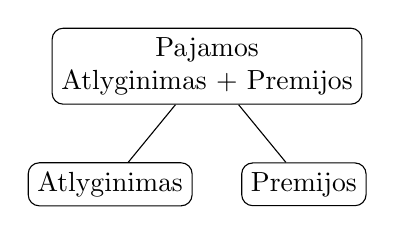
\begin{tikzpicture}[sibling distance=7em,	
            every node/.style = {shape=rectangle, rounded corners,	
                                 draw, align=center,	
                                 top color=white, bottom color=white}]	
            \node {Pajamos\\Atlyginimas + Premijos}	
                    child { node {Atlyginimas} }	
                    child { node {Premijos} } ;	
        \end{tikzpicture} 	
    \]\par
     Po tam tikro laiko atsirado poreikis pajamas skaičiuoti pagal formulę: \[\textit{Pajamos = Atlyginimas + Premijos + Komandiruočių dienpinigiai}\] Naujas rodiklių medis atrodys taip: 
     \[	
        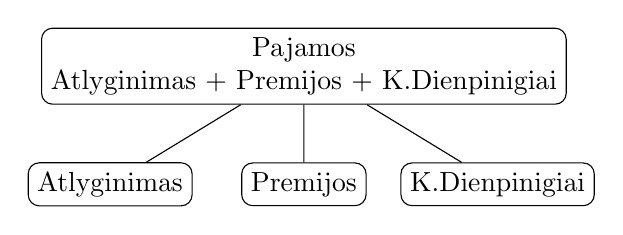
\begin{tikzpicture}[sibling distance=7em,	
            every node/.style = {shape=rectangle, rounded corners,	
                                 draw, align=center,	
                                 top color=white, bottom color=white}]	
            \node {Pajamos\\Atlyginimas + Premijos + K.Dienpinigiai}	
                    child { node {Atlyginimas} }	
                    child { node {Premijos} } 
                    child { node {K.Dienpinigiai} };	
        \end{tikzpicture} 	
    \]
\end{itemize} 

\noindent 
\section{Srautinio duomenų apdorojimo sprendimų analizė}

\subsection{Srautinis duomenų apdorojimas} \label{strprocess}

Siekiant apžvelgti modernius srautinio duomenų apdorojimo sprendimus šiame skyriuje apsibrėžiamos jų savybes.
2005 metais Michael Stonebraker apibrėžė 8 taisykles realaus laiko (angl. real-time) srautinio duomenų apdorojimo architektūrai \cite{stonebraker20058}:
\begin{enumerate}[label=\arabic*]
    \item taisyklė: Duomenys turi judėti. Žemo uždelstumo užtikrinimui sistema turi apdoroti duomenis nenaudojant duomenų saugojimo operacijų. 
    Taip pat sistema turi ne pati užklausti duomenų, o gauti juos iš kito šaltinio asinchroniškai. 
    \item taisyklė: Duomenų transformacijos turi būti vykdomas SQL pobūdžio užklausomis. Žemo abstrakcijos lygmens srautinio apdorojimo sistemos reikalauja ilgesnio programavimo laiko ir brangesnio palaikymo. Tuo tarpu aukšto abstrakcijos lygmens sistema naudojanti SQL užklausas, kurias žino dauguma programuotojų ir yra naudojamos daugelyje skirtingų sistemų, leidžia efektyviau kurti srautinio apdorojimo sprendimus.
    \item taisyklė: Architektūra turi susidoroti su duomenų netobulumais. Architektūra turi palaikyti galimybę nutraukti individualius skaičiavimus tam, kad neatsirastų blokuojančių operacijų, kurios sustabdo vieno modulio veikimą ir tuo pačiu visos architektūros veikimą. Taip pat ši architektūra turi sugebėti susidoroti su vėluojančiomis žinutėmis, pratęsiant laiko tarpą, per kurį ta žinutė turi ateiti.
    \item taisyklė: Architektūra turi būti deterministinė. Kiekvieną kartą apdorojant tuos pačius duomenis rezultatai turi būti gaunami tokie patys.
    \item taisyklė: Architektūra turi gebėti apdoroti išsaugotus duomenis ir realiu laiku gaunamus duomenis. Sistema parašyta su tokia architektūra turi galėti apdoroti jau esančius duomenis taip pat kaip ir naujai ateinančius. Toks reikalavimas buvo aprašytas, nes atsirado poreikis nepastebimai perjungti apdorojimą iš istorinių duomenų į realiu laiku ateinančius duomenis automatiškai.
    \item taisyklė: Architektūra turi užtikrinti duomenų saugumą ir apdorojimo prieinamumą. Kadangi sistema turi apdoroti didelius kiekius duomenų, architektūra klaidos atveju, turi sugebėti persijungti į atsarginę sistemą ir tęsti darbą toliau. Taip pat tokios klaidos atveju atsarginė sistema turi būti apdorojusi visus duomenis ir sugebėti iš karto priimti naujus duomenis, o ne apdoroti duomenis iš pradžių.
    \item taisyklė: Architektūra turi užtikrinti sugebėjimą paskirstyti sistemos darbus automatiškai. Srautinio apdorojimo sistemos turi palaikyti kelių procesoriaus gijų operacijas. Taip pat sistema turi galėti veikti ant kelių kompiuterių vienu metu ir prireikus paskirstyti resursus pagal galimybes.
    \item taisyklė: Architektūra turi apdoroti ir atsakyti akimirksniu. Anksčiau minėtos taisyklės nėra svarbios, jeigu sistema nesugeba greitai susidoroti su dideliu kiekiu naujų duomenų. Todėl turi būti naudojamas ne tik teisingas ir greitas srautinio apdorojimo sprendimas, bet ir gerai optimizuota sistema.
\end{enumerate}\par 
Todėl norint sužinoti tam tikro srautinio duomenų apdorojimo sprendimo tinkamumą uždaviniui reikia išanalizuoti jų savybes.   
\subsection{Srautinio duomenų apdorojimo sistemos}

Norime nustatyti srautinio apdorojimo sistemų savybes pagal:
\begin{itemize}
    \item Pristatymo semantika (angl. delivery semantics) - apibrėžia pagal kokį modelį bus pristatyti duomenys. Egzistuoja trys semantikos \cite{ensar20}: 
    \begin{itemize}
        \item Bent vieną kartą (angl. at-least-once) užtikrina, kad duomenys bus apdoroti bent kartą, bet gali atsirasti dublikatų. 
        \item Ne daugiau vieno karto (angl. at-most-once) užtikrina, kad duomenys bus apdoroti daugiausiai tik vieną kartą, bet gali atsirasti praradimų. 
        \item Tiksliai vieną kartą (angl. exactly-once) užtikrina, kad duomenys bus apdoroti tik vieną kartą ir klaidos bus suvaldytos.
    \end{itemize}
    \item Uždelstumas (angl. latency) - apibrėžia laikų sumą - kiek laiko trūko viena operacija ir kiek laiko ši operacija turėjo laukti eilėje kol bus pabaigtos kitos operacijos \cite{karimov2018benchmarking}.
    \item Pralaidumas (angl. throughput) - apibrėžia kiek pavyks įvykdyti operacijų per tam tikrą laiko tarpą.
    \item Abstrakcijos lygmuo (angl. abstraction) - apibrėžia kokio lygmens programavimo sąsają pateikia sprendimas.
\end{itemize}
Tam išnagrinėsime ir palyginsime, kaip šitas savybes išpildo keturi egzistuojantys srautinio apdorojimo sprendimai - "Apache Storm", "Apache Spark", "Apache Flink" ir "Heron".

\subsection{Pristatymo semantika}
"Apache Spark" ir "Apache Flink" sprendimų pristatymo semantika yra tiksliai vieną kartą (angl. exactly-once), tai reiškia, kad visi duomenys bus apdoroti tik vieną kartą. Tačiau tam, kad užtikrinti šią semantiką sprendimas sunaudoja daug resursų, kadangi reikia užtikrinti, kad operacija bus vykdoma būtent vieną kartą kiekviename srautinio apdorojimo žingsnyje: duomenų gavime, kuris stipriai priklauso nuo duomenų šaltinio, duomenų transformacijos, kurią turi įvykdyti srautinio apdorojimo sprendimas, ir duomenų saugojime, tai turi būti užtikrinta sprendimo ir naudojamos saugyklos \cite{zhang20}.\par

"Apache Storm" pristatymo semantika yra bent vieną kartą (angl. at-least-once), tai reiškia, kad į šį sprendimą siunčiami duomenys bus visada apdoroti, tačiau kartais gali būti apdoroti kelis kartus \cite{prithi20}. Jei uždavinys nereikalauja tiksliai vieno karto apdorojimo, tai geriau rinktis bent vieną kartą ar ne daugiau vieno karto semantikas, kadangi jos neturi papildomų apsaugų, kurios reikalingos tiksliai vieno karto apdorojimui, ir todėl veikia greičiau \cite{zhang20}. \par

"Heron" sprendimų pristatymo semantika gali būti keičiama, programuotojas kuriantis srautinio apdorojimo sistemą šiam sprendimui aprašo kokio tipo pristatymo semantikos kuriama sistema reikalauja \cite{delivery-semantics}.

\subsection{Uždelstumas}

Uždelstumas - laiko trukmė, kuri parodo kaip greitai sprendimas įvykdo vieną operaciją, nuo jos patekimo į eilę iki šios operacijos apdorojimo pabaigos. Pagal \cite{Lopez2016APC} aprašytus Martin Andreoni Lopez "Apache Storm", "Apache Spark" ir "Apache Flink" bandymus galima matyti, kad būtent "Apache Storm" turi mažiausią uždelstumą. Kadangi parinkus tinkamą paralelizmo parametrą šis sprendimas su užduotimi susidorojo net iki 15 kartų greičiau. Antroje vietoje liko "Apache Flink", o po jos "Apache Spark". \par

"Heron" sprendimas yra sukurtas siekiant pagerinti "Apache Storm" sprendimo greitaveika, todėl jo uždelstumas yra dar mažesnis nei "Apache Storm" \cite{Kulkarni:2015:THS:2723372.2742788}.

\subsection{Pralaidumas}

Pralaidumas apibrėžia kokį kiekį procesų sprendimas gali įvykdyti per tam tikrą laiko tarpą. 2016 metais Sanket Chintapalli išmatavo "Apache Storm", "Apache Spark" ir "Apache Flink" sprendimų pralaidumą ir uždelstumą bei palygino rezultatus. Kaip ir anksčiau manyta, "Apache Spark" turėjo aukščiausia pralaidumą iš visų, kadangi jis vienintelis duomenis apdoroja mikro-paketais\cite{chintapalli2016benchmarking}. Antroje vietoje liko "Apache Flink", kuris yra subalansuotas pralaidumo atžvilgiu ir paskutinis liko "Apache Storm", kuris turi žemą uždelstumą, todėl nukenčia pralaidumas. "Heron" tuo tarpu turi aukštesnį pralaidumą ir žemesnį uždelstumą nei "Apache Storm" \cite{TwitterHeron}. 

\subsection{Abstrakcijos lygmuo}

"Apache Storm" parašytos sistemos yra žemo abstrakcijos lygmens, tai reiškia, kad turi būti aprašyti visi srautinio apdorojimo moduliai: 
setSpouts(..), kuriame nustatoma duomenų įeiga ir koks bus paralelizmo lygis, setBolt(..), kuriame nustatomi apdorojimo moduliai, kokius duomenis gaus iš prieš tai buvusio modulio ir paralelizmo lygis. Kiekvieno modulio execute() metodas aprašo, kaip šis modulis turi apdoroti duomenis \cite{tutpoint}. Šio sprendimo programų kūrimo laikas užtruks ilgiau negu kitiems sprendimams su aukštu abstrakcijos lygmeniu, tačiau žemas abstrakcijos leidžia rašyti daug greičiau veikiančias sistemas, kadangi programuotojas turi pilną kontrolę. \par

"Apache Spark" parašytos programos yra aukšto abstrakcijos lygmens. Sistemos aprašomos funkciškai, todėl kodo rašymas trunka daug trumpiau ir jį yra daug lengviau skaityti. Tačiau prarandama galimybė optimizuoti ir paralelizmo klausimas paliekamas sprendimui. Kadangi "Apache Spark" yra ne pilnai srautinis, o mikro-paketinis (angl. micro-batching) sprendimas, todėl vartotojas turi apsirašyti kokio dydžio paketais bus renkami duomenys \cite{shoro2015big}. \par

"Apache Flink" parašytos programos yra aukšto abstrakcijos lygmens. "Apache Flink" sprendimas pats užsiima resursų distribucija, todėl programuotojui lieka tik parašyti veikianti kodą, o sistema pati susitvarkys su paralelizmu \cite{flinkdoc}. Tačiau tai reiškia, kad su šiuo sprendimu parašytos programos nepavyks optimizuoti taip pat gerai kaip žemo abstrakcijos lygmens sistemos. \par

"Heron" sprendimas turi skirtingus API, kurie naudoja skirtingus abstrakcijos lygius, kuriuos galima rinktis pagal tinkamumą sprendžiamai problemai. Darbo rašymo metu "Heron" turi 4 skirtingus API:
\begin{itemize}
    \item "Heron Streamlet API" - aukšto abstrakcijos lygmens API, rašomas su "Java" programavimo kalba. Panaši sintaksė į "Apache Flink" rašomų sprendimų.
    \item "Heron ECO API" - eksperimentinis aukšto abstrakcijos lygmens API, rašomas su "Java" programavimo kalba. Skiriasi nuo "Heron Streamlet API", nes modulių apdorojimo eiliškumas apsirašo YAML formatų, kas leidžia keisti sukurtos srautinio duomenų apdorojimo programos struktūrą nekeičiant kodo.
    \item "Heron Topology API for Java" - žemo abstrakcijos lygmens API, rašomas su "Java" programavimo kalba. Rašomas identiškas kodas, kaip ir "Apache Storm", kadangi "Heron" sprendimas buvo sukurtas siekiant pagerinti "Apache Storm".
    \item "Heron Topology API for Python" - žemo abstrakcijos lygmens API, rašomas su "Python" programavimo kalba. Su šiuo API kuriami srautinio apdorojimo sprendimai yra panašus į "Apache Storm", tik su "Python" programavimo kalbos privalumais.
\end{itemize}  


\subsection{Apibendrinimas}

Pagal atlikta analizę, sudaryta \ref{table:comparer} lentelė. Iš šių keturių sprendimų pasirinktas vienas, kuris labiausiai tinka rodiklių duomenų srautinio apdorojimo sistemų generavimui, pagal aprašytas savybes. Tinkamas sprendimas turi pasižymėti: 
\begin{itemize}
    \item Apdorojimo greičiu, svarbu, kad duomenys būtų apdorojami kai tik patenka į sistemą, todėl turi būti žemas uždelstumas.
    \item Tiksliai vieną kartą apdorojimu, kadangi norint gauti tikslius rodiklių duomenis turi neišsikreipti pirminių rodiklių duomenų aibė apdorojimo metu.
    \item Žemu abstrakcijos lygiu, nes tai leidžia generuoti iš anksto optimizuotas srautinio apdorojimo sistemas.  
\end{itemize} 

\begin{table}[!htbp]
    \begin{center}
        \caption{Srautinių duomenų apdorojimo sprendimų palyginimas}
        \label{table:comparer}
        \begin{tabular}{ | l | c | c | c | c | }
            \hline
            \cellcolor[gray]{0.8} Charakteristika & \cellcolor[gray]{0.9} "Apache Storm" & \cellcolor[gray]{0.9} "Apache Spark" & \cellcolor[gray]{0.9} "Apache Flink" & \cellcolor[gray]{0.9} "Heron" \\* \hline
            \cellcolor[gray]{0.9} Pristatymas & Bent vieną kartą & Tiksliai vieną kartą & Tiksliai vieną kartą & Pasirenkamas \\* \hline
            \cellcolor[gray]{0.9} Uždelstumas & Žemas & Aukštas & Vidutinis & Žemas \\* \hline
            \cellcolor[gray]{0.9} Pralaidumas & Žemas & Aukštas & Vidutinis & Vidutinis \\* \hline
            \cellcolor[gray]{0.9} Abstrakcijos lygis & Žemas & Aukštas & Aukštas & Pasirenkamas \\* \hline
        \end{tabular}
    \end{center}
\end{table}\par

Pagal analizę (\ref{table:comparer} lentelė.) ir apsibrėžtus reikalavimus darbe sprendžiamam uždaviniui tinkamiausias srautinio apdorojimo sprendimas yra "Heron". \par

\section{Srautinio duomenų apdorojimo sistemų architektūra}

Šiame skyriuje apžvelgiamas srautinio apdorojimo sistemų rašymas "Heron" sprendimui ir srautinio apdorojimo sistemų generavimas pagal deklaratyviai aprašyta rodiklių duomenų modelį.

\subsection{Srautinio apdorojimo sistemos komponentai}
"Heron" sprendimui parašytos srautinio apdorojimo sistemos susidaro iš trijų tipų komponentų:
\begin{itemize}
    \item "Spout" - duomenų įeigos komponentas. Gali būti daugiau nei vienas, jeigu yra daugiau nei vienas duomenų šaltiniai, pavyzdžiui, žinučių eilė ir duomenų bazė.
    \item "Bolt" - duomenų apdorojimo komponentas. Gali būti daugiau nei vienas. Gali gauti duomenis iš "Spout" komponentų ir iš kitų "Bolt" komponentų.
    \item "Topology" aprašo skirto aprašyti srautinio apdorojimo sistemos pavadinimą, konfigūracijas (pristatymo semantika, kontrolinių saugojimo tašku intervalas ir t.t.) ir specifikuoti, kaip tarpusavyje sujungti "Spout" ir "Bolt" komponentai ir jų paralelizmo lygis. 
\end{itemize}
Konkretus pavyzdys srautinio apdorojimo sistemos atrodo taip:
Reikalinga srautinio apdorojimo sistema, kuriai bus siunčiami sakiniai, o ji gražins žodyną su žodžių dažniu. Vienas iš būdų įgyvendinti tokią sistemą (\ref{img:example}. pav) yra:
\begin{itemize}
    \item Įeigos "Spout" komponentas gaunantis sakinius iš žinučių eilės ir perduodantis(angl. emit) sakinius toliau.
    \item Skaidymo "Bolt" komponentas gaunamus sakinius suskaidantis į žodžius ir perduodantis juos toliau.
    \item Skaičiavimo "Bolt" komponentas saugantis pasikartojančių žodžių žodyną, kur raktas - žodis, o reikšmė - kiek kartų pasikartojo. Gavęs žodi jis padidina jo skaitiklį žodyne ir perduoda žodyną į "Rezultatų" žinučių eilę.
\end{itemize}
\begin{figure}[H]
    \centering
    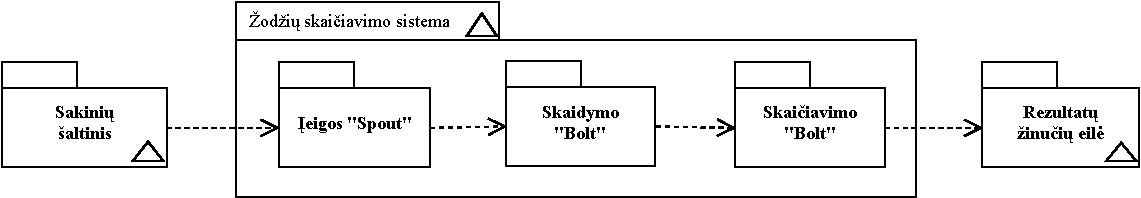
\includegraphics[width=1\textwidth]{img/pavyzdine_sistema.pdf}
    \caption{Srautinio apdorojimo sistemos pavyzdys}
    \label{img:example}
\end{figure}

\subsection{Srautinio apdorojimo sistemų sudarymas pagal rodiklių duomenų modelį}
Srautinio apdorojimo sistemos sudarytos pagal deklaratyvų rodiklių duomenų modelį atrodo taip:
\begin{enumerate}
    \item "Spout" tipo įeigos komponentas. Šis komponentas aprašo priminių rodiklių duomenų filtravimo predikatus ir pirminį raktą. 
    \item "Bolt" tipo komponentai, kurie sudaryti pagal rodiklių duomenų modelio rodiklius. Kiekvienam rodikliui turi būti vienas "Bolt" tipo komponentas. "Bolt" komponentai gali būti dviejų tipų:
    \begin{itemize}
        \item Paprastų rodiklių "Bolt" komponentai, kurie atsakingi už pirminių rodiklių duomenų apdorojimą.
        \item Išvestiniai rodiklių "Bolt" komponentai, kurie atsakingi už duomenų, gautų iš paprastų arba išvestinių rodiklių "Bolt" komponentų, transformaciją. Transformacijos - bet kokie iš anksto aprašyti nuoseklus veiksmai su duomenų rinkiniu gražinantys vieną rezultatą. Pavyzdžiui: norint sudaryto išvestinį rodiklį, kuris skaičiuoja dviejų pirminių rodiklių sumą turi būti:
        \begin{itemize}
            \item Iš anksto aprašyta funkcija "suma", kuri priima du skaičius ir gražina vieną.
            \item Rodiklio modelyje užrašyta transformacija - suma(rodiklis1, rodiklis2).
        \end{itemize} 
    \end{itemize}
    \item "Topology" aprašas, kuriame aprašomos "Spout" ir "Bolt" komponentų jungimaisi tarpusavyje pagal priklausomybių medžiu iš rodiklių duomenų modelio.
\end{enumerate}
Pavyzdžiui, jei rodiklis atrodo taip:     
\[
    \begin{tikzpicture}[sibling distance=10em,
        level distance=2cm,
        every node/.style = {shape=rectangle, rounded corners,	
                             draw, align=center,	
                             top color=white, bottom color=white}]	
        \node{Žmonių kaita\\Nuolatinė kaita + (Migracija * Gyventojų kiekis)}
                child { node {Nuolatinė kaita\\Gimstamumas - Mirtingumas} 
                        child {node {Mirtingumas}}
                        child {node {Gimstamumas}} }	
                child { node {Migracija} } 	
                child { node {Gyventojų kiekis} }; 	
    \end{tikzpicture} 	
\]\par
"Heron" sprendimui sukurta srautinio apdorojimo sistema atrodys taip:
\begin{figure}[H]
    \centering
    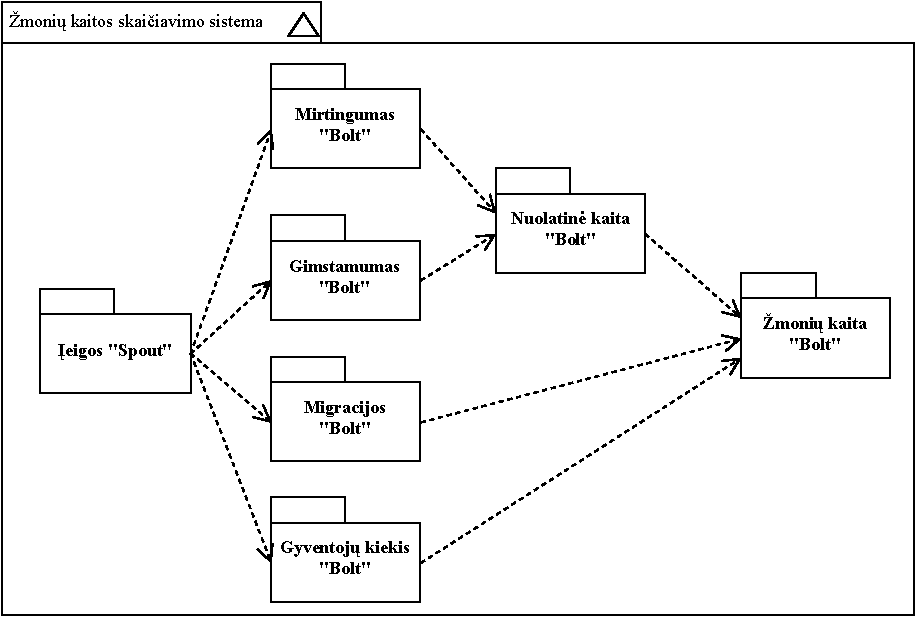
\includegraphics[width=1\textwidth]{img/generuota_sistema.pdf}
    \caption{Srautinio apdorojimo sistemos pavyzdys}
    \label{img:example}
\end{figure}

\section{Eksperimentas ir sukurto sprendimo savybės}

\subsection{Eksperimento tikslas}

Eksperimento tikslas - sukurti koncepcinį sprendimą, kurio pagalba patikrinti, ar sudaryta architektūra išpildo šias savybes:
\begin{itemize}
    \item Srautinių apdorojimo sistemų generavimas pagal deklaratyvų aprašymą.
    \item Galimybė keisti esamas apdorojimo sistemas, kai pakeičiamas rodiklių duomenų modelis.
    \item Išvestinių rodiklių gavimas iš daugiau nei vieno rodiklio transformacijos.
    \item Išvestinių rodiklių apdorojimas pagal iš anksto apibrėžtas funkcijas.
\end{itemize}  

\noindent Siekiant tai patikrinti su sukurtu sprendimu atlikti šie bandymai:
\begin{enumerate}
    \item Sukurtas pavyzdinis rodiklių duomenų modelis, aprašytas deklaratyviai ir pateiktas į koncepcinį sprendimą.
    \item Atnaujintas rodiklių duomenų modelis (pridėtas naujas išvestinis rodiklis) ir pateiktas į koncepcinį sprendimą.
\end{enumerate}

\subsection{Eksperimento vykdymo aplinka}

Kompiuterio, kuriame buvo vykdomas eksperimentas specifikacijos:
\begin{itemize}
    \item Procesorius - Intel Core i7-7700k 4,5GHz
    \item Sisteminis diskas -  512 GB SSD
    \item Operatyvioji atmintis - 16 GB 
    \item Operacinė sistema - Ubuntu 18.04
\end{itemize}

\subsection{Koncepcinis sprendimas}

Siekiant nustatyti sudarytos architektūros savybes sukurtas koncepcinis sprendimas (\ref{img:concept} pav.). Sudarytas iš šių pagrindinių komponentų:
\begin{itemize}
    \item Sistemų generavimo komponentas - programa generuojanti srautinio apdorojimo sistemas.
    \item Duomenų bazės komponentas - duomenų bazė sauganti rodiklių duomenų apdorojimo rezultatus
    \item Srautinio apdorojimo sprendimas - programinė įranga, kurioje veikia sugeneruotos srautinio apdorojimo sistemos.
\end{itemize}

\begin{figure}[H]
    \centering
    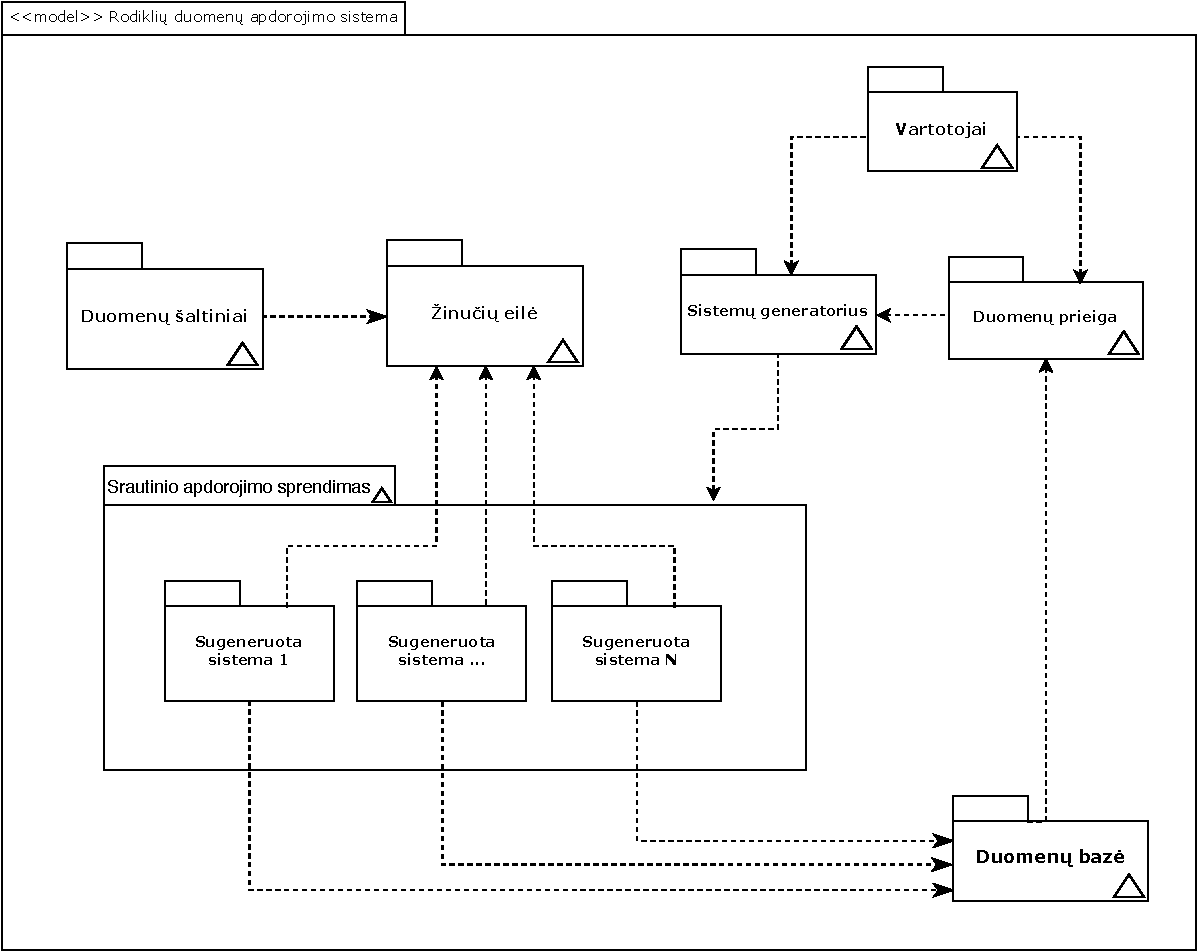
\includegraphics[width=0.8\textwidth]{img/architekturos_diagrama.pdf}
    \caption{Koncepcinio sprendimo architektūra}
    \label{img:concept}
\end{figure}

\subsubsection{Sistemų generavimo komponentas}

Sistemų generavimo komponentas - programa sukurta su ".NET core" biblioteka, nes reikalingas taškas (angl. endpoint) deklaratyviai aprašyto rodiklio modelio pateikimui. Srautinio apdorojimo sistemų kodo generavimas yra vykdomas pagal šablonus, kurie sukurti kiekvienam srautinio apdorojimo sprendimo komponento tipui. Šablono laukai, kuriuos reikia pakeisti, užrašyti specialiais identifikuojančiais elementais. Generavimo metu šie elementai keičiami reikiamu kodu užduočiai spręsti.
Šiame komponente kodo generavimas veikia taip (\ref{img:generation-flow} pav.):

\begin{enumerate}
    \item Gaunamas rodiklių duomenų modelis.
    \item Tikrinama ar jau egzistuoja tokia srautinio apdorojimo sistema. Tai daroma kreipiantis į duomenų bazę ir tikrinant, ar egzistuoja įrašų, kurių raktai sutampa su generuojamos sistemos pavadinimu.
    \item Jei egzistuoja:
        \begin{enumerate}
            \item Sustabdoma veikianti sistemą. Tai vykdoma kviečiant stabdymo komandą per Ubuntu operacinės sistemos terminalą.
            \item Iš duomenų bazės ištraukiami jau apdorotus rodiklių duomenis ir perduodami į generavimo dalį.
        \end{enumerate} 
    \item Generuojamas srautinio apdorojimo sistemos įeigos "Spout" tipo komponentą. Jame įrašomas žinučių eilės grupės pavadinimą, sąlygas pirminių rodiklių duomenims pagal apribojimus ir pirminių rodiklių duomeniui sugeneruojamas unikalus identifikatorius, kurio pagalba išvestinių rodiklių apdorojimo komponentas vykdo išskaičiavimus duomenis teisinga tvarka.
    \item Pagal rodiklius generuojami duomenų apdorojimo "Bolt" tipo komponentai. Jeigu generuojamas komponentas jau egzistuoja, sugeneruotas rodiklio apdorojimo "Bolt" tipo komponento kodas užpildomas rezultatais gautais iš duomenų bazės. 
    \item Generuojamas sistemos "Topology" tipo aprašas, kuriame įrašyta komponentų jungimosi tarpusavyje logiką ir kitos sistemos konfigūracijas. 
    \item Visas sugeneruotas kodas talpinamas į vieną aplanką ir sukompiliuojamas "Pants" programinės įrangos pagalba.
    \item Sukompiliuota sistema pateikiama į srautinio apdorojimo programą.
\end{enumerate}

\begin{figure}[H]
    \centering
    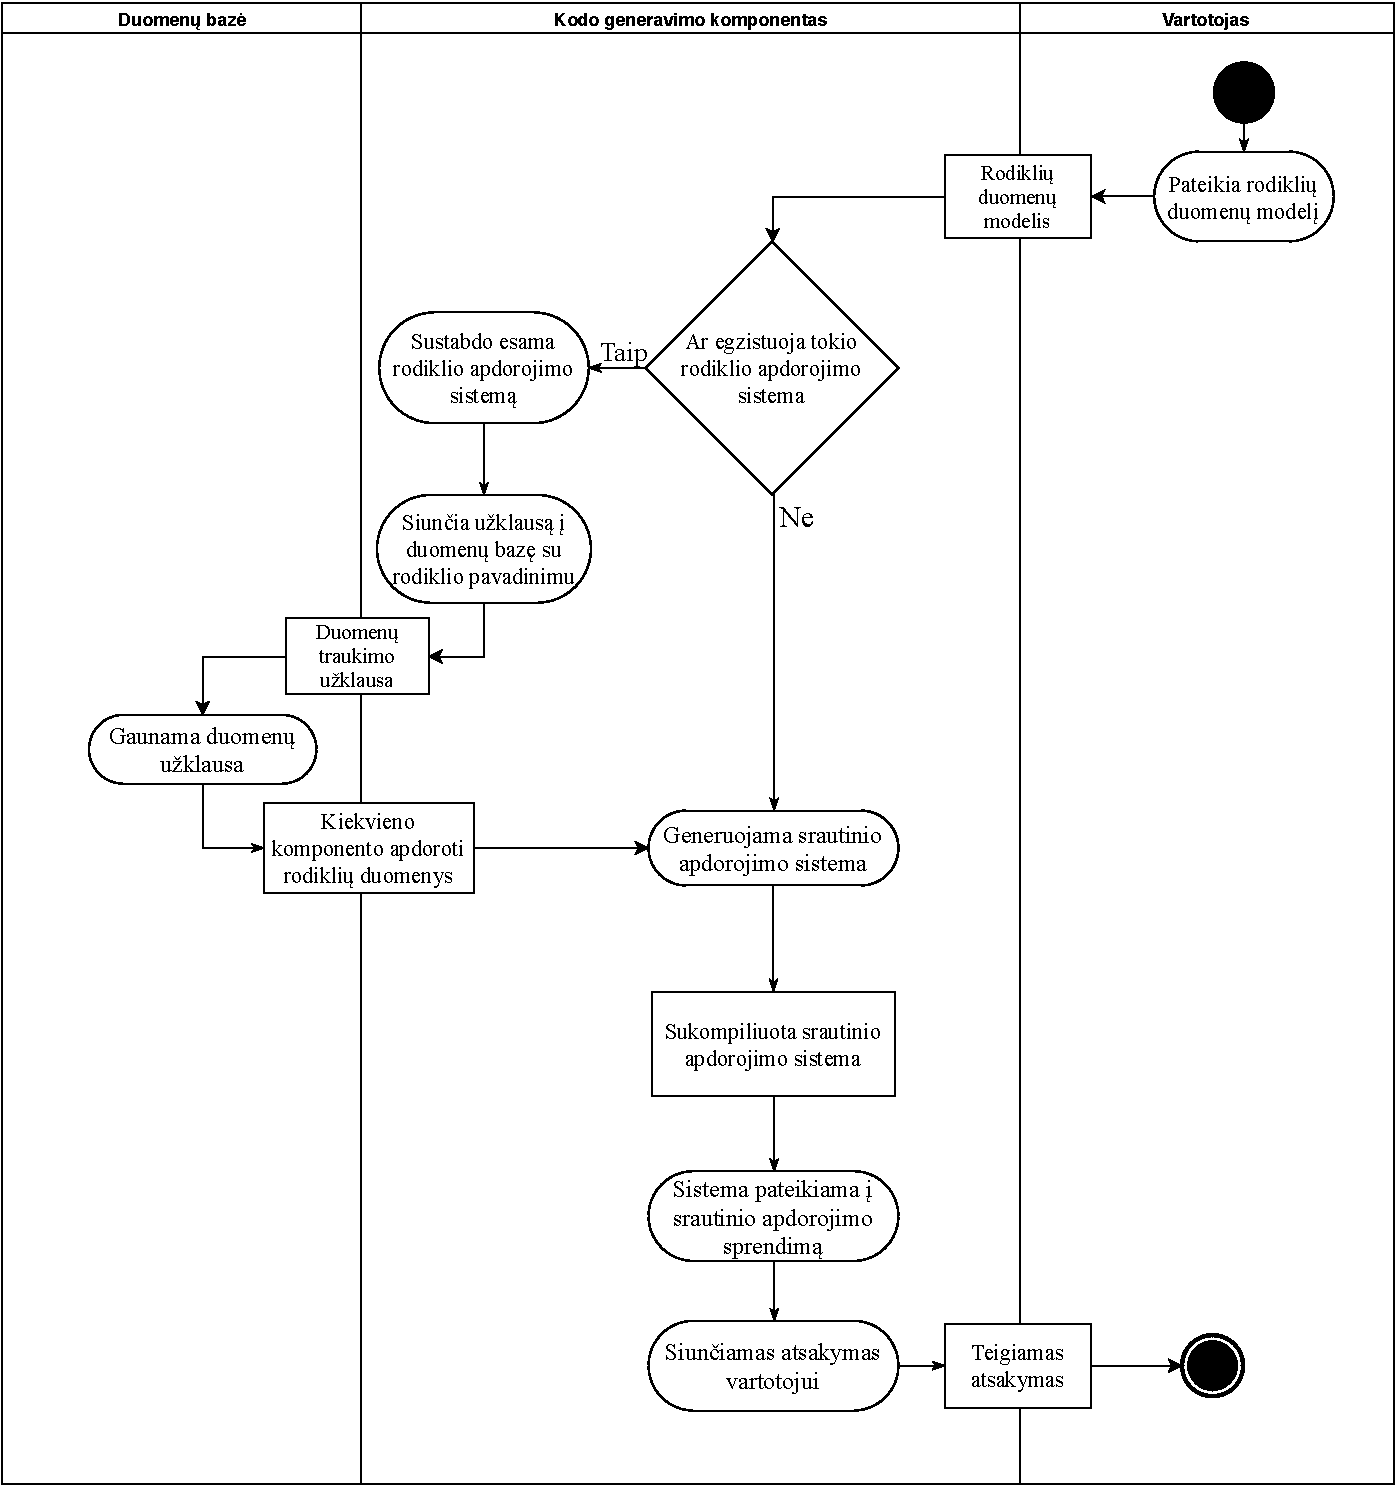
\includegraphics[width=0.8\textwidth]{img/generation-flow.pdf}
    \caption{Srautinio apdorojimo sistemų generavimo komponento veikimas}
    \label{img:generation-flow}
\end{figure}

\subsubsection{Apdorotų rodiklių duomenų bazė}

Duomenų bazė koncepciniam sprendime saugo apdorotus rodiklių duomenis. Norint saugoti apdorotus išvestinių ir pagrindinių rodiklių duomenis, visi srautinio apdorojimo sistemų komponentai yra prijungti prie duomenų bazės ir apdoroję duomenis talpina juos į duomenų bazę perrašydami ten jau esamus. Duomenys iš duomenų bazės naudojami dviem poreikiam: 
\begin{enumerate}
    \item Gauti apdorotus rodiklių duomenis. Siunčiant užklausą su srautinio apdorojimo sistemos pavadinimu į koncepciniam sprendime sukurta tašką  gražinamas atsakymas su apdorotais rodikliais. 
    \item Srautinio apdorojimo sistemų generavimo komponentas rezultatų duomenų gavimui. Kadangi po rodiklių pridėjimo arba pašalinimo apdorojimas turi vykti toliau, po srautinio apdorojimo sistemos sustabdymo, kodo generavimo komponentas trauks rezultatus ir dės juos į atnaujintos srautinio apdorojimo sistemos nepakitusius komponentus.   
\end{enumerate}  

Saugoti apdorotus duomenis buvo pasirinkta "Redis" duomenų bazę. Ji pasirinkta kadangi apdoroti rodiklių duomenis užima nedaug vietos, o labai svarbu greitai pasiekti ir įdėti duomenis. "Redis" duomenų bazių valdymo sistema tinka, nes duomenis saugomi operatyvioje atmintyje, kas leidžia duomenis ištraukti ir įdėti greičiau nei tradicinėse duomenų bazėse \cite{carlson2013redis}.\par
Apdoroti rodikliai saugomi unikalioje eilėje pagal srautinės apdorojimo sistemos ir rodiklio pavadinimų kombinaciją. Pavyzdžiui: renkant darbuotojų atlyginimus per metus pagal uždarbio ir premijos kombinaciją, apdoroti rodiklių duomenys būtų saugomi pagal raktus: "darbuotojų-atlyginimas:uždarbis", "darbuotojų-atlyginimas:premijos" ir "darbuotojų-atlyginimas:atlyginimas"

\subsubsection{Papildoma programinė įranga}

Koncepcinio sprendimo veikimui taip pat reikia papildomos programinės įrangos, kurį užsiima duomenų perdavimu, srautinio apdorojimo sistemų kompiliavimu.
\begin{itemize}
    \item Žinučių eilės pagrindinis uždavinys - perduoti duomenis į srautinio apdorojimo sistemą. Žinučių eilės naudoja publikavimo-prenumeratos modelį (angl. publish-subscribe pattern), komponentai norintys gauti duomenis užsiregistruoja žinučių eilėje, o komponentai siunčiantis tiesiog perduoda juos į žinučių eilę. Taip yra įgyvendinamas asinchroninis bendravimas, komponentai perduoda duomenis į žinučių eilę, o komponentas norintis gauti duomenis gali juos pasiimti bet kuriuo momentu iš eilės. Koncepcinio sprendimo įgyvendinimui pasirinkta Apache Kafka žinučių eilė.
    \item Apache Kafka reikalauja Apache Zookeeper, kuris atsakingas už Apache Kafka žinučių eilės konfigūracijos valdymą.
    \item Sugeneruotos sistemos kompiliavimui naudojama "Pants" kompiliavimo sistema.
\end{itemize}
Taip pat norint eksperimentų atlikimui yra reikalinga programinė įranga:
\begin{itemize}
    \item Pirminių rodiklių duomenų siuntimo komponentas. Šis Python kalba parašytas komponentas į žinučių eilę reguliaru intervalu siunčia duomenis sugeneruotus su \url{https://mockaroo.com/} įrankiu.
    \item Postman programinė įranga, kuri naudojama išsiųsti rodiklių duomenų modelį į koncepcinio sprendimo generavimo tašką.
    \item Naršyklė, kuri naudojama stebėti sugeneruotas ir pateiktas srautinio apdorojimo sistemas per "Heron" sąsają ir gauti duomenis iš apdorotų rodiklių duomenų bazės.
\end{itemize}

\subsection{Eksperimentas}

Eksperimento vykdymui sudarytas rodiklių duomenų uždavinys: išmanus ofisas turi sensorius - drėgmės, temperatūros, šviesos. Poreikis surinkti valandinius dienos (nuo 8 valandos iki 20 valandos) pagal kabineto numerį rodiklius. Taip pat norima apskaičiuoti išvestinį juntamosios temperatūros rodiklį pagal formulę\cite{anderson2013methods}: 
\[\textit{Juntamoji temperatūra} = \textit{Temperatūra} – (0.55 * (1 –\>\frac{\textit{Drėgmė}}{1000}) * (\textit{Temperatūra} – 14.5))\]
Taip pat tarkime, kad po laiko buvo nuspręsta pridėti naują bendro pojūčio išvestini rodikli, kuris išskaičiuojamas taip: 
\[\textit{Bendras pojūtis} = \frac{\textit{Šviesumas}}{75} * \frac{\textit{Juntamoji temperatūra}}{25} \]

\subsubsection{Pradiniai duomenys}
\noindent Pradinis rodiklių duomenų modelis pagal uždavinį atrodo taip:
\begin{itemize}
    \item Pirminis raktas: \(\textit{"Valanda", "Kabinetas"}\)
    \item Pirminių rodiklių duomenų apribojimai: \(\textit{"Valanda" > 7},\textit{"Valanda" < 21}\) 
    \item Rodikliai:
    \[
        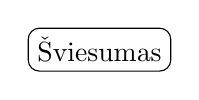
\begin{tikzpicture}[sibling distance=10em,
            level distance=2cm,
            every node/.style = {shape=rectangle, rounded corners,	
                                draw, align=center,	
                                top color=white, bottom color=white}]	
            \node{Šviesumas}; 	
        \end{tikzpicture}\>\>\>\>
        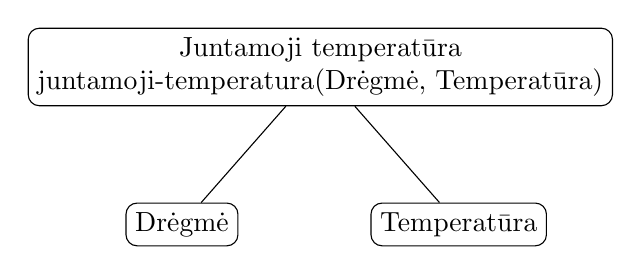
\begin{tikzpicture}[sibling distance=10em,
            level distance=2cm,
            every node/.style = {shape=rectangle, rounded corners,	
                                draw, align=center,	
                                top color=white, bottom color=white}]	
            \node{Juntamoji temperatūra\\juntamoji-temperatura(Drėgmė, Temperatūra)}
                    child { node {Drėgmė} }	
                    child { node {Temperatūra} } ; 	
        \end{tikzpicture} 	
    \]
\end{itemize}
Atnaujintas rodiklių duomenų modelis atrodo taip:
\begin{itemize}
    \item Pirminis raktas: \(\textit{"Valanda", "Kabinetas"}\)
    \item Pirminių rodiklių duomenų apribojimai: \(\textit{"Valanda" > 7},\textit{"Valanda" < 21}\) 
    \item Rodikliai:
    \[	
        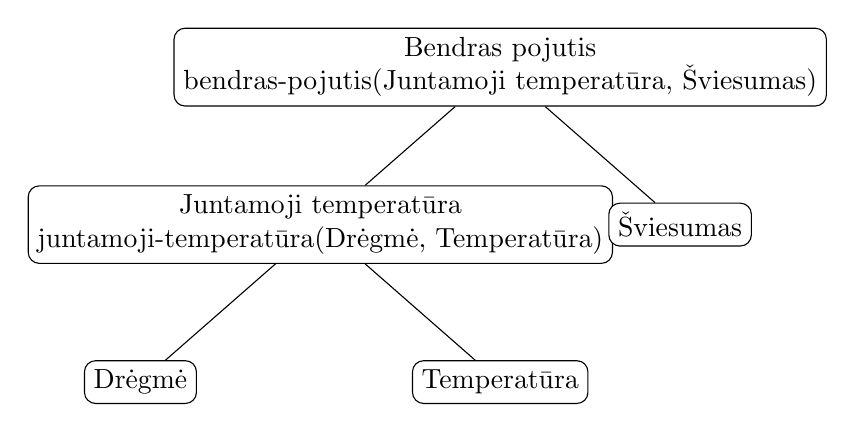
\begin{tikzpicture}[sibling distance=13em,
            level distance=2cm,
            every node/.style = {shape=rectangle, rounded corners,	
                                draw, align=center,	
                                top color=white, bottom color=white}]	
            \node{ Bendras pojutis \\bendras-pojutis(Juntamoji temperatūra, Šviesumas)}
                child{ node {Juntamoji temperatūra\\juntamoji-temperatūra(Drėgmė, Temperatūra)}
                        child { node {Drėgmė} }	
                        child { node {Temperatūra} } }
                child {node {Šviesumas}}; 	
        \end{tikzpicture} 	
    \]
\end{itemize}

\noindent Taip pat sugeneruoti pirminiai rodiklių duomenys naudojant \url{https://mockaroo.com/} įrankį (Priedas \ref{add:mockaroo}). Šių duomenų raktai atrodo taip:
\begin{itemize}
    \item Kabineto numeris - reikšmės iš aibės - 100, 101, 102, 103, 104
    \item Valanda - reikšmės nuo 0 iki 24
    \item Drėgmė - reikšmes nuo 0 iki 100
    \item Temperatūra - reikšmės nuo 10 iki 30
    \item Šviesumas - reikšmės nuo 0 iki 100 
\end{itemize}

\subsubsection{Eksperimento eiga}

Eksperimentas buvo vykdomas tokia eiga:
\begin{enumerate}
    \item Pradinių rodiklių duomenų modelis užrašomas JSON formatu (Priedas \ref{add:initial-json}) ir naudojant Postman programą paduodamas į sprendimą.
    \item Atsidarius "Heron" sąsają naršyklėje matoma sugeneruotos srautinio apdorojimo sistemos diagramą (Priedas \ref{add:generated-system1}).
    \item Su pirminių rodiklių duomenų siuntimo programa duomenis siunčiami į žinučių eilę.
    \item Naršyklėje išsiunčiama užklausa į sprendimo duomenų prieigos tašką ir gaunami apdorotus rodiklių duomenys (Priedas \ref{add:generated-data1}).
    \item Atnaujintas rodiklių duomenų modelis užrašomas JSON formatu (Priedas \ref{add:changed-json}) ir naudojant Postman programą paduodamas į sprendimą.
    \item Atnaujinus "Heron" sąsają naršyklėje matoma, jog atsinaujino srautinio apdorojimo sistemos diagrama (Priedas \ref{add:generated-system2}).
    \item Naršyklėje siunčiama užklausa į sprendimo tašką ir gaunami apdoroti rodiklių duomenis, kuriuose jau galima matyti naujo rodiklio rezultatus(Priedas \ref{add:generated-data2}).
\end{enumerate}

\subsubsection{Eksperimento rezultatai}
Stebint eksperimentą gauti rezultatai:
\begin{itemize}
    \item Sėkmingai sugeneruota srautinio apdorojimo sistema iš rodiklio duomenų modelio.
    \item Srautinio apdorojimo sistema sėkmingai apdorojo pirminiai rodiklių duomenys pagal rodiklių duomenų modelį.
    \item Išvestinių rodiklių "Bolt" komponentai teisingai išskaičiavo rezultatus pagal iš anksto aprašytas funkcijas naudojant duomenis iš daugiau nei vieno "Bolt" komponento.
    \item Sėkmingai atnaujinta srautinio apdorojimo sistema pakeitus rodiklių duomenų modelį.
    \item Atnaujinus srautinio apdorojimo sistemą nepakeisti "Bolt" tipo komponentai toliau pratęsė rodiklių apdorojimą. 
\end{itemize}
\subsection{Sprendimo savybės}

Sukurtas koncepcinis sprendimas įrodo, jog sugeneruotos srautinio apdorojimo sistemos pagal rodiklių duomenų modelį atitinka šias savybes:
\begin{itemize}
    \item Išvestinių rodiklių išskaičiavimas iš daugiau nei vieno rodiklio kombinacijos.
    \item Išvestinių rodiklių išskaičiavimas pagal iš anksto aprašytą transformaciją.
    \item Prisitaikymas prie rodiklių duomenų struktūros pokyčių. 
    \item Nepakitusių rodiklių apdorojimo pratęsimas po rodiklių duomenų struktūros pakeitimo.
\end{itemize} 

\sectionnonum{Rezultatai}

\begin{enumerate}
    \item Apibrėžtas rodiklių duomenų modelis ir galimi duomenų struktūros pokyčiai.
    \item Atlikta srautinio apdorojimo sprendimų "Apache Storm", "Apache Spark", "Apache Flink" ir "Heron" analizė ir analizės rezultatas apibendrintai pateiktas pagal analizuotas savybes. 
    \item Sudaryta srautinio apdorojimo sistemos architektūra tinkama spręsti rodiklių apdorojimo uždavinį su "Heron" srautinių apdorojimo sprendimu. 
    \item Siekiant nustatyti ar srautinio apdorojimo architektūra atitinka apsibrėžtas savybes:
    \begin{itemize}
        \item Aprašyti bandymams naudojami rodiklių duomenų modeliai.
        \item Sukurtas koncepcinis sprendimas \url{http://gitlab.com} generuojantis srautinio apdorojimo sistemas pagal aprašytą architektūrą.
        \item Su koncepciniu sprendimu atliktas srautinės rodiklių duomenų apdorojimo sistemos generavimo eksperimentas. 
    \end{itemize} 
\end{enumerate}

\sectionnonum{Išvados}
\begin{enumerate}
    \item Rodiklių duomenų modelis turi susidaryti iš trijų dalių:
    \begin{itemize}
        \item Pirminio rakto - rodiklių duomenų grupavimui
        \item Apribojimų rinkinio - pirminių rodiklių duomenų filtravimui
        \item Rodiklių rinkinio, kur rodiklių tarpusavio priklausomybės sudaro priklausomybių medį - rodiklių apdorojimo specifikacijai.
    \end{itemize}
    \item Rodiklių duomenis apdorojančioms srautinio apdorojimo sistemom generuoti geriausiai tinka "Heron" srautinio apdorojimo sprendimas, nes rodiklių duomenų apdorojimui svarbus žemas uždelstumas, kad būtų užtikrintas apdorojimo greitis, tiksliai vieną kartą apdorojimas, kad nebūtų prarandami duomenys apdorojimo metu ir žemas abstrakcijos lygis, kad būtų galima generuoti optimizuotas srautinio apdorojimo sistemas.
    \item Rodiklių duomenų uždaviniui spręsti srautinių apdorojimo sistemų kūrimui gali būti naudojamas srautinio apdorojimo sistemų generavimas, kadangi tai suteikia galimybę kurti srautinio apdorojimo sistemas iš deklaratyviai aprašyto rodiklių duomenų modelio.
    \item Eksperimento būdų įrodyta, jog siūlomas srautinio apdorojimo sistemų generavimas pagal deklaratyvų rodiklių duomenų modelį gali būti įgyvendinamas. Sugeneruotos srautinio apdorojimo sistemos atitinka apsibrėžtas savybės, kurių reikia rodiklių duomenų apdorojimui. Įrodyta, jog srautinių apdorojimo sistemų generavimas "Heron" srautinio apdorojimo sprendimui yra tinkamas rodiklių duomenų apdorojimo uždaviniui spręsti.  
\end{enumerate}

\printbibliography[heading=bibintoc] 

\appendix 

\section{Pirminių rodiklių duomenų generavimo įrankis}\label{add:mockaroo}
\begin{figure}[H]
    \centering
    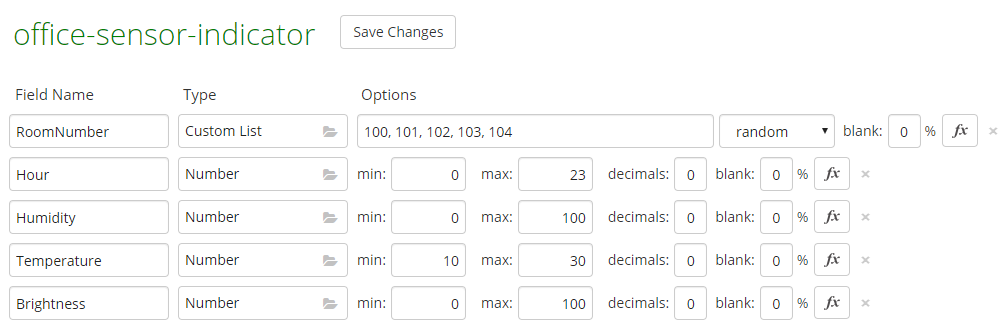
\includegraphics[width=1\textwidth]{img/generated-data.png}
    \label{img:generated-data}
\end{figure}

\section{Rodiklių duomenų modelis JSON formatu}\label{add:initial-json}
\lstset{
    string=[s]{"}{"},
    stringstyle=\color{blue},
    comment=[l]{:},
    commentstyle=\color{black},
    breaklines=true
}
\begin{lstlisting}
{
    "IndicatorId": "32c24420-afbd-44fb-b045-ef72c48cb04e",
    "Name": "office-sensors-indicator",
    "VersionId": "1-416f51b5-2b8a-4cb0-9978-f713d5990c52",
    "PrimaryKey": [
        "RoomNumber",
        "Hour"
    ],
    "Filters": [
        {
            "FieldName": "Hour",
            "Value": 7,
            "Operator": "MORE"
        },
        {
            "FieldName": "Hour",
            "Value": 21,
            "Operator": "LESS"
        }
    ],
    "Values": [
        {
            "Id": "5dbfcf52-bbce-4ec6-ad31-1cf0812b3106",
            "FieldName": "HeatIndex",
            "Formula": "%65c89c44-f5c5-48d4-ba31-01e3d4b69e42% - (0.55 * (1 - (%117af450-3086-412f-90f5-ad63e1989d04%/1000)) * (%65c89c44-f5c5-48d4-ba31-01e3d4b69e42% - 14.5))",
            "NextValues": [
                {
                    "Id": "65c89c44-f5c5-48d4-ba31-01e3d4b69e42",
                    "FieldName": "Temperature"
                },
                {
                    "Id": "117af450-3086-412f-90f5-ad63e1989d04",
                    "FieldName": "Humidity"
                }
            ]
        },
        {
            "Id": "252606d7-9b72-42d5-8923-ac8bce4f60e5",
            "FieldName": "Brightness"
        }
    ]
}
\end{lstlisting}

\section{Sugeneruota srautinio apdorojimo sistema "Heron" sąsajoje}\label{add:generated-system1}
\begin{figure}[H]
    \centering
    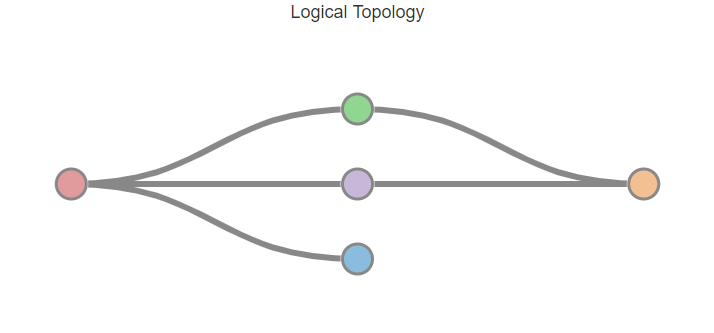
\includegraphics[width=1\textwidth]{img/generated-topology-1.png}
    \label{img:generated-data}
\end{figure}

\section{Sugeneruotos srautinio apdorojimo sistemos rezultatai}\label{add:generated-data1}
\begin{figure}[H]
    \centering
    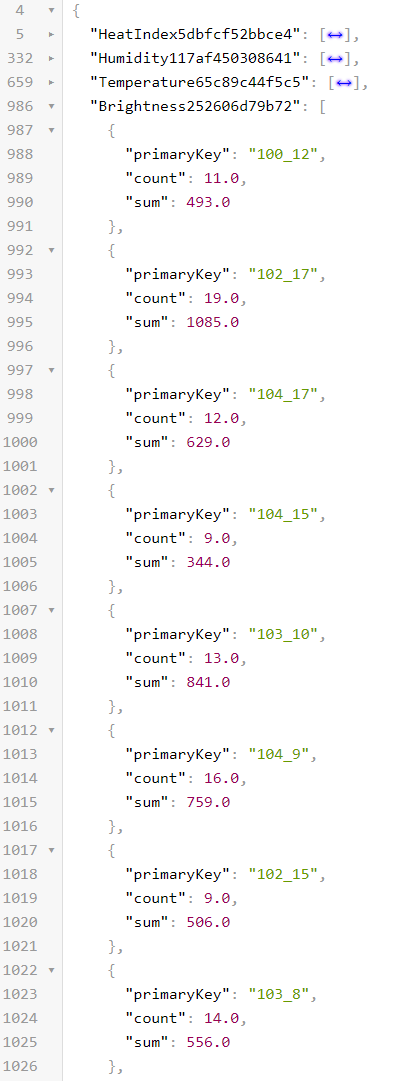
\includegraphics[width=0.5\textwidth]{img/topology-data-1.png}
    \label{img:generated-data}
\end{figure}

\section{Atnaujintas rodiklių duomenų modelis JSON formatu}\label{add:changed-json}
\begin{lstlisting}
{
    "IndicatorId": "32c24420-afbd-44fb-b045-ef72c48cb04e",
    "Name": "office-sensors-indicator",
    "VersionId": "2-a4c42274-65e9-4e9d-863b-671d51d702cf",
    "PrimaryKey": [
        "RoomNumber",
        "Hour"
    ],
    "Filters": [
        {
            "FieldName": "Hour",
            "Value": 7,
            "Operator": "MORE"
        },
        {
            "FieldName": "Hour",
            "Value": 21,
            "Operator": "LESS"
        }
    ],
    "Values": [
        {
            "Id": "5dbfcf52-bbce-4ec6-ad31-1cf0812b3106",
            "FieldName": "GeneralIndex",
            "Formula": "(%252606d7-9b72-42d5-8923-ac8bce4f60e5% / 75) * (%5dbfcf52-bbce-4ec6-ad31-1cf0812b3106% / 25)",
            "NextValues": [
                {
                    "Id": "5dbfcf52-bbce-4ec6-ad31-1cf0812b3106",
                    "FieldName": "HeatIndex",
                    "Formula": "%65c89c44-f5c5-48d4-ba31-01e3d4b69e42% - (0.55 * (1 - (%117af450-3086-412f-90f5-ad63e1989d04%/1000)) * (%65c89c44-f5c5-48d4-ba31-01e3d4b69e42% - 14.5))",
                    "NextValues": [
                        {
                            "Id": "65c89c44-f5c5-48d4-ba31-01e3d4b69e42",
                            "FieldName": "Temperature"
                        },
                        {
                            "Id": "117af450-3086-412f-90f5-ad63e1989d04",
                            "FieldName": "Humidity"
                        }
                    ]
                },
                {
                    "Id": "252606d7-9b72-42d5-8923-ac8bce4f60e5",
                    "FieldName": "Brightness"
                }
            ]
        }
    ]
}
\end{lstlisting}


\section{Atnaujintos srautinio apdorojimo sistemos "Heron" sąsajoje}\label{add:generated-system2}
\begin{figure}[H]
    \centering
    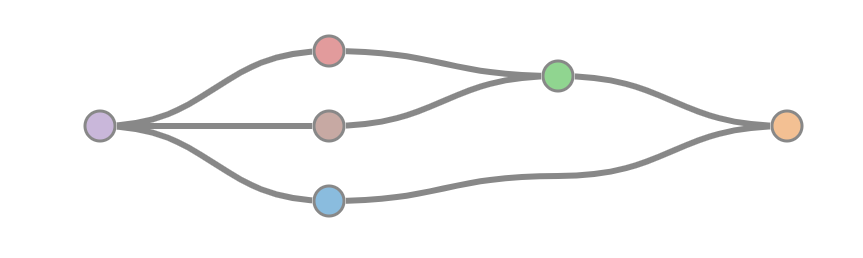
\includegraphics[width=1\textwidth]{img/generated-topology-2.png}
    \label{img:generated-data}
\end{figure}

\section{Atnaujintos srautinio apdorojimo sistemos rezultatai}\label{add:generated-data2}
\begin{figure}[H]
    \centering
    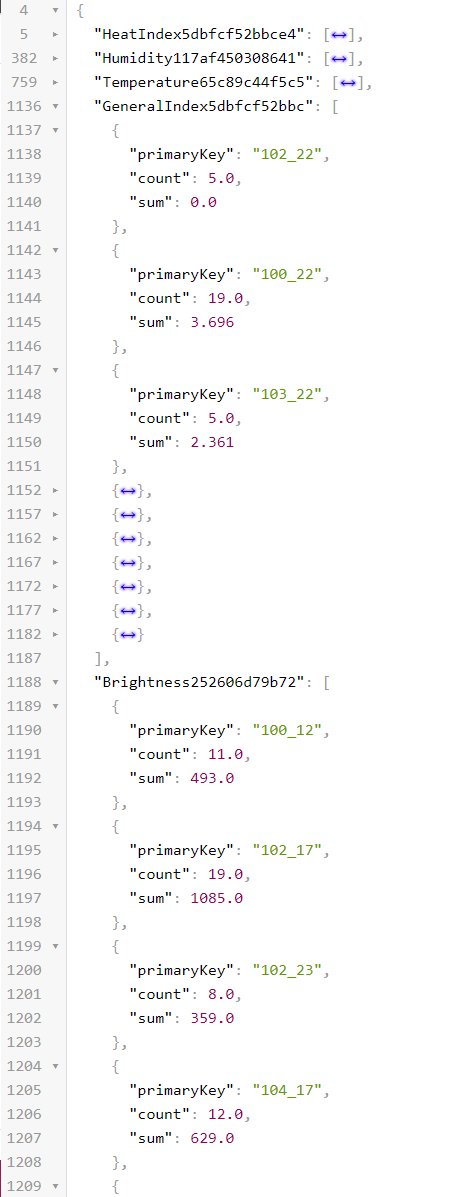
\includegraphics[width=0.5\textwidth]{img/topology-data-2.png}
    \label{img:generated-data}
\end{figure}

\end{document}
